\documentclass[11pt,letterpaper]{report}
\usepackage[latin1]{inputenc}
\usepackage{amsmath}
\usepackage{amsfonts}
\usepackage{amssymb}
\usepackage{graphicx}
\usepackage{color}
\usepackage{enumitem}
\usepackage[dvipsnames]{xcolor}
\definecolor{codegray}{gray}{0.9}
\newcommand{\code}[1]{\colorbox{codegray}{\texttt{#1}}}
\graphicspath{{./images/}{IR}}
%\newcommand{\LF}{}  % turn on to display large format
\ifdefined \LF
\usepackage[left=2.0cm, top=2.0cm, landscape]{geometry}  % for large format landscape
\else
\usepackage[left=2.0cm, top=2.0cm]{geometry}
\fi
\usepackage{fancyhdr}
\pagestyle{fancy}
\fancyhead{}
\lhead{CS333}
\chead{Project 4 Test Report}
\rhead{Alexander DuPree}
\begin{document}
\title{Project 4 Test Report}
\author{Alexander DuPree}

\ifdefined \LF
{\Large     % large print start
\fi

  \maketitle
  \section*{Introduction}
  \noindent
  The following test report documents the tests performed for project four. The test cases and strategies closely follow the project four rubric. 

  Each section contains test cases related to the sections topic. Each test case will describe the name of the test, 
  the expected result, actual result, as well as a discussion and indication of the Pass/Fail status. 
  The actual result will be provided in the form of a screen shot of the console. 

  \section*{Compilation}
  This section presents all tests related to compiling the xv6 kernel.
  Test cases follow closely those outlined in the rubric. \hfill \break
  
  \noindent\textbf{Test Case:} \emph{With CS333\_PROJECT set to 0 in the Makefile}
  
  \noindent\textbf{Assertions:}
  \begin{enumerate}[]
  \item Code correctly compiles
  \item Kernel successfully boots
  \item \code{usertests} run to completion with all tests passed
  \end{enumerate}  
  
  \noindent\textbf{Status:} \textcolor{ForestGreen}{\textbf{PASS}}
  
  \begin{figure}[h!]
	\centering
	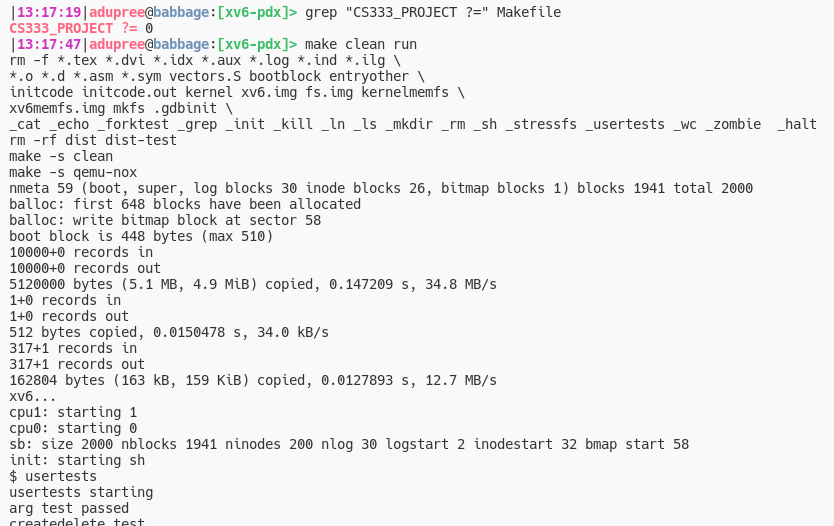
\includegraphics[width=1\linewidth]{compilation1-usertests1.png}
	\caption[img]{Compilation and boot with CS333\_PROJECT set to 0 and execution of \code{usertests}}
	\label{fig:P1compileP0-1}
  \end{figure}

  \begin{figure}[h!]
	\centering
	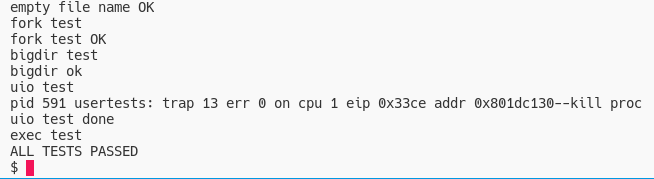
\includegraphics[width=1\linewidth]{compilation1-usertests2.png}
	\caption[img]{Completion of \code{usertests} with output elided}
	\label{fig:P1compileP0-1}
  \end{figure}

  The command \code{grep "CS333\_PROJECT ?=" Makefile} shows that the CS333\_PROJECT macro is set to 0.
  The following command \code{make clean run} demonstrates that the code correctly compiles and the kernel successfully boots. 
  Furthermore, the commands were executed within seconds of each other, indicating that
  tampering is not a possibility. Lastly, we can see that the execution of \code{usertests}
  is initiated in the same session, and Figure 2 shows that the tests run to completion and 
  all tests pass. \\

  \pagebreak

  \noindent\textbf{Test Case:} \emph{With CS333\_PROJECT set to 4 in the Makefile}
  
  \noindent\textbf{Assertions:}
  \begin{enumerate}[]
  \item Code correctly compiles
  \item Kernel successfully boots
  \item \code{usertests} run to completion with all tests passed
  \end{enumerate}  
  
  \noindent\textbf{Status:} \textcolor{ForestGreen}{\textbf{PASS}}
  
  \begin{figure}[h!]
	\centering
	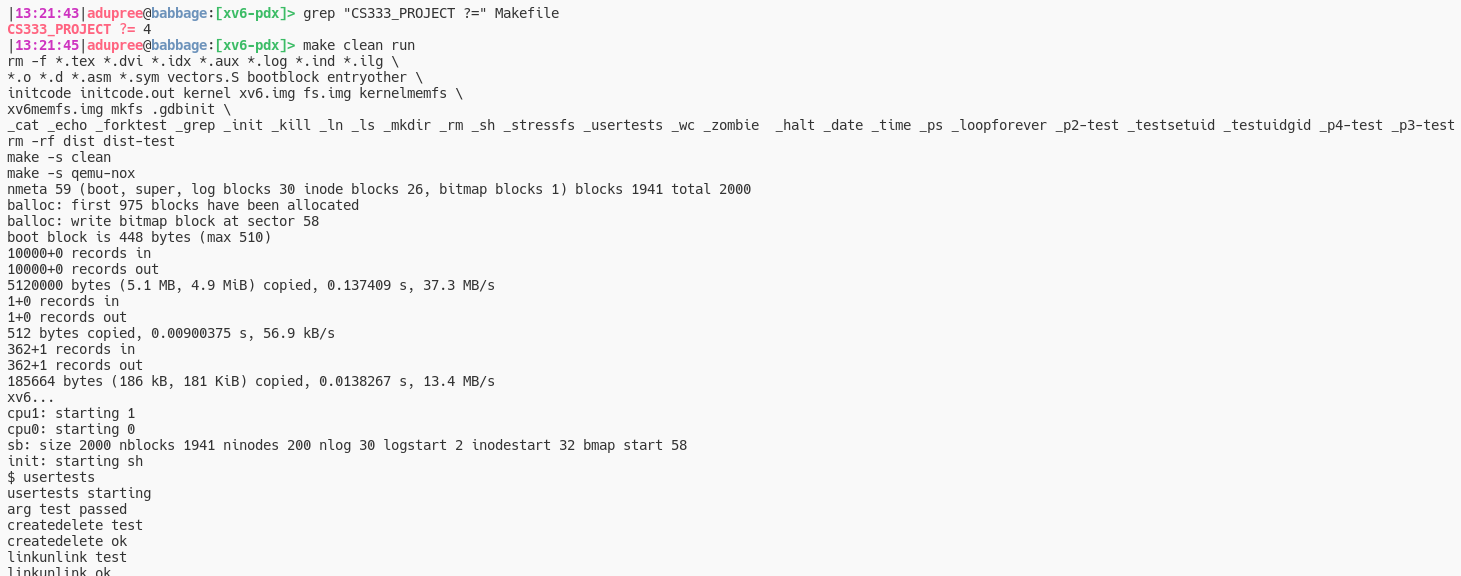
\includegraphics[width=1\linewidth]{compilation2-usertests1.png}
	\caption[img]{Compilation and boot with CS333\_PROJECT set to 4 and execution of \code{usertests}.}
	\label{fig:P1compileP0-1}
  \end{figure}

  \begin{figure}[h!]
	\centering
	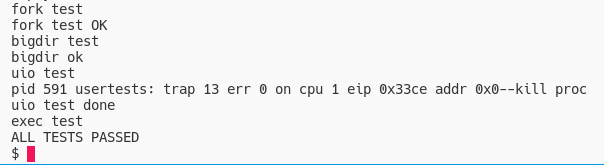
\includegraphics[width=1\linewidth]{compilation2-usertests2.png}
	\caption[img]{Completion of \code{usertests} with output elided, CS333\_P4 is defined}
	\label{fig:P1compileP0-1}
  \end{figure}

  The command \code{grep "CS333\_PROJECT ?=" Makefile} shows that the CS333\_PROJECT macro
  is indeed set to 4. The following command \code{make clean run} demonstrates that the code
  correctly compiles and the kernel successfully boots. Furthermore, the commands were executed
  within seconds of each other, indicating that tampering is not a possibility. Lastly, we can
  see that the execution of \code{usertests} is initiated in the same session and Figure 4
  demonstrates that the tests run to completion and all tests pass. \\
  
  \pagebreak

  \section*{Updated Commands}
  This section presents all tests related to the new information displayed for the 
  \code{ps} program, CTRL+P and CTRL+R interrupts. Test cases follow closely those outlined in the rubric. \hfill \break
  
  \noindent\textbf{Test Case:} \emph{CTRL+P, \code{ps} and CTRL+R}
  
  \noindent\textbf{Note:} \code{MAXPRIO} = 4, \code{DEFAULT\_BUDGET} = 10000, \code{TICKS\_TO\_PROMOTE} = 100000

  \noindent\textbf{Assertions:}
  \begin{enumerate}[]
  \item CTRL+P correctly displays all active processes and their priorities
  \item \code{ps} output matches CTRL+P, excluding program counters
  \item CTRL+R displays all ready lists, from highest to lowest priority, and the budget for each process
  \end{enumerate}  
  
  \noindent\textbf{Status:} \textcolor{ForestGreen}{\textbf{PASS}}
  
  \begin{figure}[h!]
	\centering
	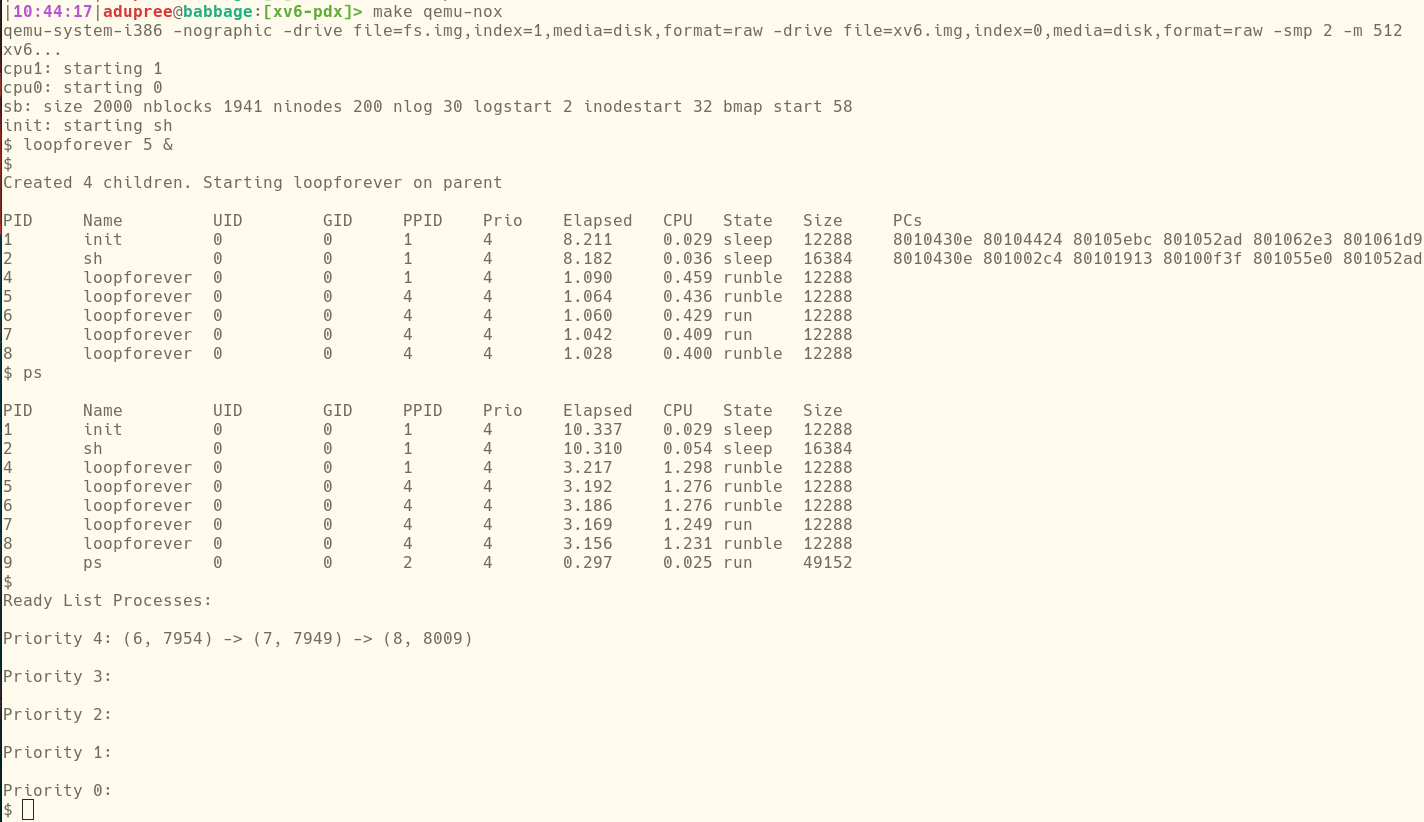
\includegraphics[width=1\linewidth]{updated-commands.png}
	\caption[img]{Output of CTRL+P, CTRL+R and the \code{ps} program}
	\label{fig:P1compileP0-1}
  \end{figure}

  The first command we run is \code{loopforever 5 \&} to get 5 processes that will take turns
  on the ready list in the background. Then we use the CTRL+P interrupt, as we can see in 
  figure 5 it properly displays the priority of each process. In this case the budget is set so
  high that each process will stay in the \code{MAXPRIO} queue. Then we run the \code{ps}
  program, which matches the output of CTRL+P. Finally, we use CTRL+R to display the ready lists.
  In figure 5, three of the five background processes (the other 2 are running) are on the max priority ready list and their budgets are all 
  less than the \code{DEFAULT\_BUDGET} which was 10000.

  \section*{Set and Get Priority}
  This section presents all tests related to the set and get priority system calls. These 
  tests make use of the \code{setpriority} and \code{getpriority} user programs which 
  simply take the command line args, forward them to the correct system call and report 
  the pass/fail status. Test cases follow closely those outlined in the rubric. \hfill \break

  \noindent\textbf{Test Case:} \emph{getpriority}
  
  \noindent\textbf{Note:} \code{MAXPRIO} = 3, \code{DEFAULT\_BUDGET} = 100000, \code{TICKS\_TO\_PROMOTE} = 1000000
  I.E. No promotions or demotions during this test.

  \noindent\textbf{Assertions:}
  \begin{enumerate}[]
  \item Retrieves correct priority for the relevant process
  \item Returns an error PID is not found
  \end{enumerate}  

  \noindent\textbf{Status:} \textcolor{ForestGreen}{\textbf{PASS}}
  
  \begin{figure}[h!]
	\centering
	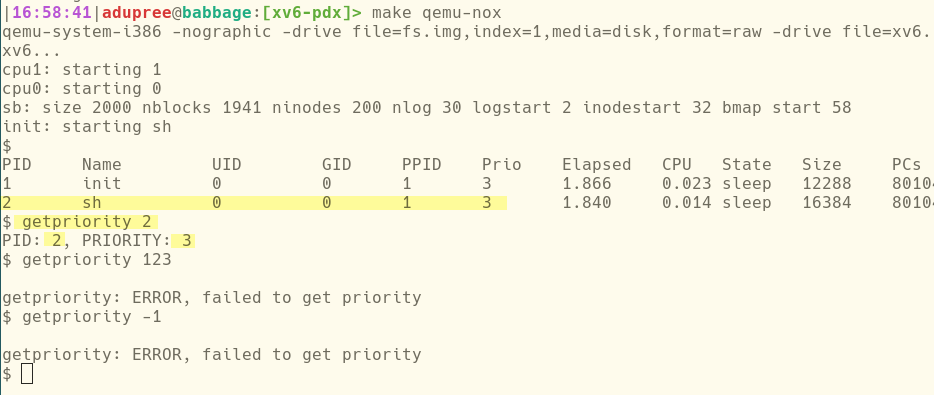
\includegraphics[width=1\linewidth]{get-priority.png}
	\caption[img]{Getting priority of processes}
	\label{fig:P1compileP0-1}
  \end{figure}

  Because the On startup we use CTRL+P to display the current processes. As we can see the priority of the 
  \code{sh} process is 3. Calling \code{getpriority 2} returns the expected value of 3. Furthermore, 
  attempting to call \code{getpriority} with PID's that don't exist or are out of bounds results in 
  an error. 

  \pagebreak

  
  \noindent\textbf{Test Case:} \emph{setpriority}
  
  \noindent\textbf{Note:} \code{MAXPRIO} = 3, \code{DEFAULT\_BUDGET} = 100000, \code{TICKS\_TO\_PROMOTE} = 1000000

  \noindent\textbf{Assertions:}
  \begin{enumerate}[]
  \item setpriority changes the priority and resets the budget
  \item Setting the priority of a process on a ready list to the same priority it already
        has does not change the position in the list for that process
  \item Calling setpriority() with an invalid PID and/or priority returns an error and leaves the 
        process priority and budget unmodified
  \end{enumerate}  
  
  \noindent\textbf{Status:} \textcolor{ForestGreen}{\textbf{PASS}}
  
  \begin{figure}[h!]
	\centering
	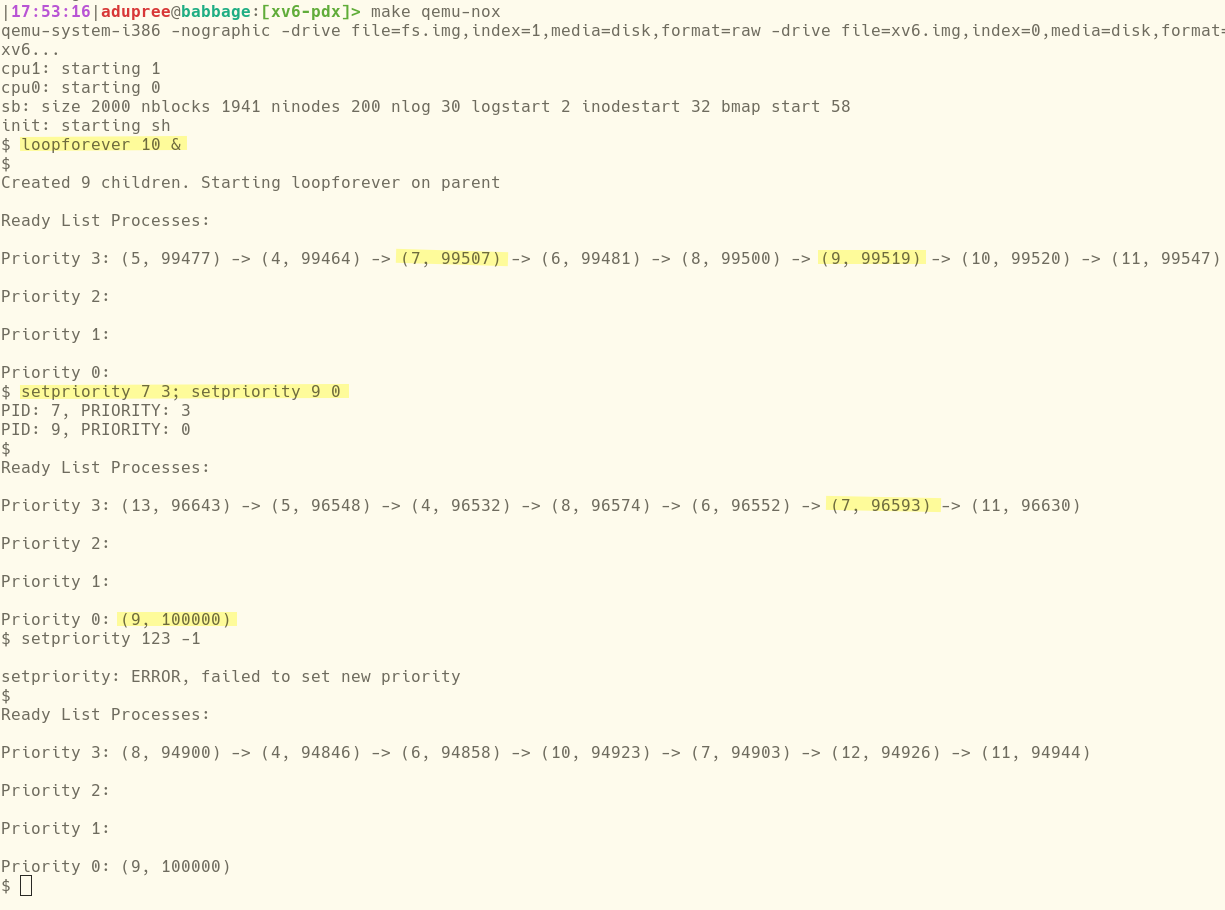
\includegraphics[width=1\linewidth]{setpriority.png}
	\caption[img]{Output of CTRL+P, CTRL+R and the \code{ps} program}
	\label{fig:P1compileP0-1}
  \end{figure}

  The first command we run is \code{loopforeer 10 \&}, which instantiates 10 processes that'll 
  loop forever in the background. Next we use CTRL+R to display the current state of the ready
  lists. Since the \code{DEFAULT\_BUDGET} and \code{TICKS\_TO\_PROMOTE} are set so high, the 
  MLFQ will essentially run in round robin order with the max priority queue. Then we call 
  \code{setpriority 7 3}, which attempts to set process \code{7} to its current priority, 
  and \code{setpriority 9 0} which will demote process \code{9} to the lowest priority. The 
  subsequent use of CTRL+R shows that prorcess \code{9} was indeed set to 0 and it's budget was
  reset to the default value. We can also see that process \code{7} did not change lists and its
  budget was not reset (since its budget is roughly the same as everyone elses in the queue).
  Lastly, we call \code{setpriority 123 -1} to generate an error and CTRL+R to show that processes
  did not have their priority or budget arbitrarily modified. 
  
  \pagebreak

  \section*{Multi-Level-Feedback Queue}
  This section presents all tests related to operation of the Multi-Level-Feedback Queue 
  scheduler algorithm. Test cases follow closely those outlined in the rubric. \hfill \break
  
  \noindent\textbf{Test Case:} \emph{With MAXPRIO set to 0}
  
  \noindent\textbf{Note:} \code{MAXPRIO} = 0, \code{DEFAULT\_BUDGET} = 1000, \code{TICKS\_TO\_PROMOTE} = 10000

  \noindent\textbf{Assertions:}
  \begin{enumerate}[]
  \item Scheduler operates as a single round-robin queue
  \item \code{setpriority} for any value other than 0 fails
  \item No promotion of demotion occurs
  \end{enumerate}  
  
  \noindent\textbf{Status:} \textcolor{ForestGreen}{\textbf{PASS}}\\
  
  \begin{figure}[h!]
	\centering
	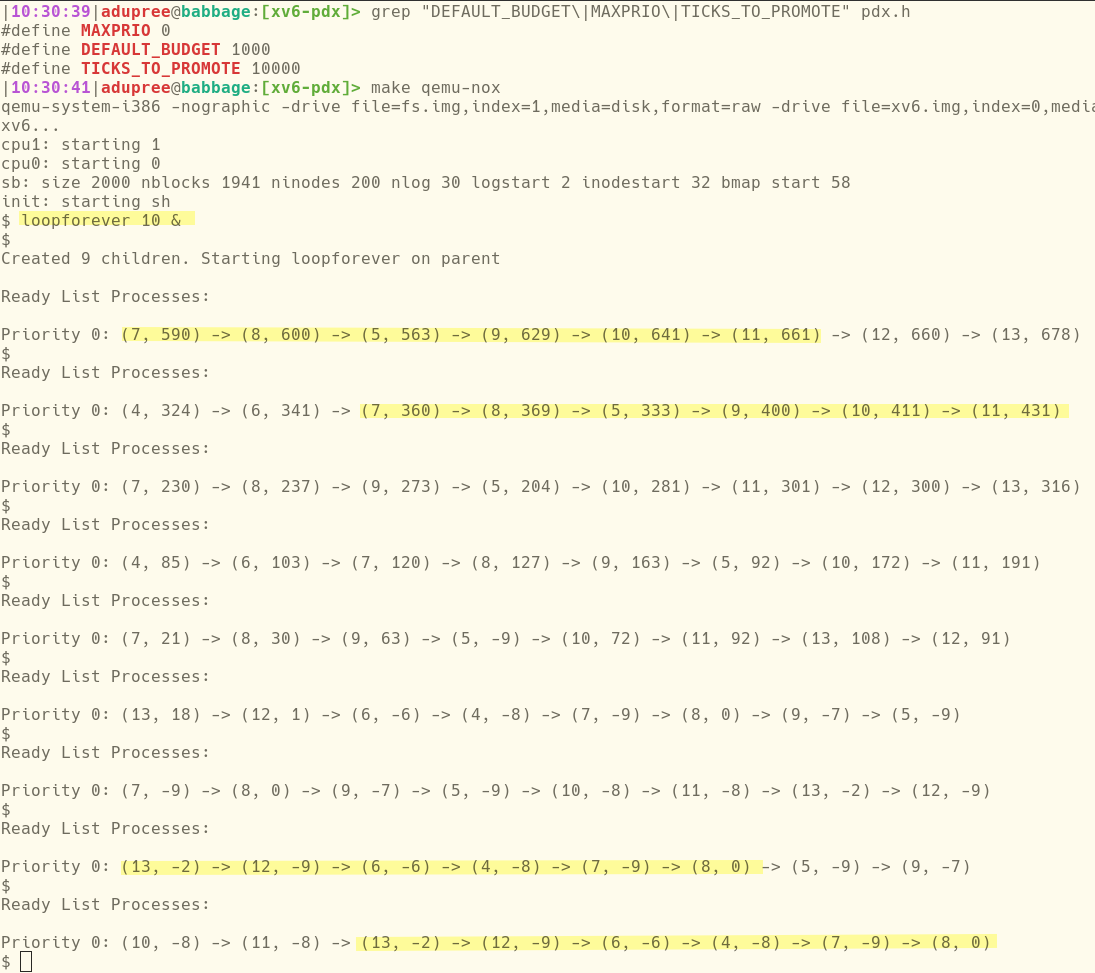
\includegraphics[width=1\linewidth]{maxprio-0.png}
	\caption[img]{Holding down CTRL+R with \code{MAXPRIO} set to 0}
	\label{fig:P1compileP0-1}
  \end{figure}

  \begin{figure}[h!]
	\centering
	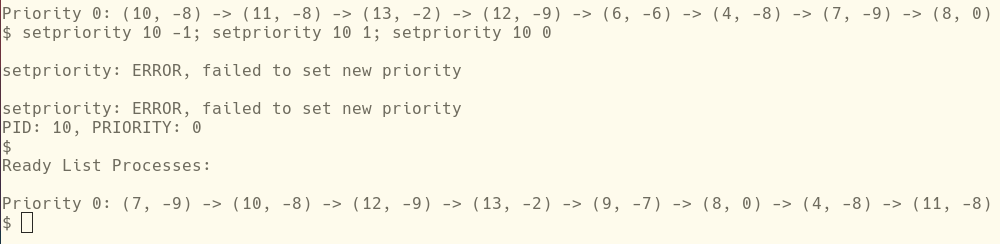
\includegraphics[width=1\linewidth]{maxprio-0-set.png}
	\caption[img]{\code{setpriority} fails for any value other than 0}
	\label{fig:P1compileP0-1}
  \end{figure}

  First, the command \code{grep "DEFAULT\_BUDGET\\|MAXPRIO\\|TICKS\_TO\_PROMOTE" pdx.h} is performed
  to verify that the kernel constants are indeed set to 1000, 0, and 10000 respectively. On 
  kernel boot the first thing we do is run \code{loopforever 10 \&} to get 10 runnable processes
  to loop forever in the background. Then, we hold down the CTRL+R interrupt to display how the 
  MLFQ scheduler is utilizing the ready lists. First we notice that since \code{MAXPRIO} is 0 
  there is only one ready list. Because there is only one ready list the scheduler acts as a 
  single round-robin queue with no promotion or demotions occuring. The highlighted 
  sections of Figure 8 below presents chains of processes that move from the front of the 
  queue to the back of the queue and maintain their order which is evidence of the round-robin
  algorithm. Furthermore, we can see the budgets bottom out at or below a zero value and are 
  no longer updated. Because no promotion/demotion occurs the budgets for each value are no longer
  reset. Lastly, in Figure 9 we attempt to set the priority of process \code{10} in three different 
  ways. Attempting to set the priority to any value other than 0 caused an error. 

  \pagebreak

  \noindent\textbf{Test Case:} \emph{With MAXPRIO set to 2}
  
  \noindent\textbf{Assertions:}
  \begin{enumerate}[]
  \item Scheduler always selects the first process on the highest priority non-empty list
  \item Promotion correctly moves processes to the next higher priority list. 
  \item Demotion correctly moves a process to the next lower priority list.
  \end{enumerate}  
  
  \noindent\textbf{Status:} \textcolor{ForestGreen}{\textbf{PASS}}\\
  
  \begin{figure}[h!]
	\centering
	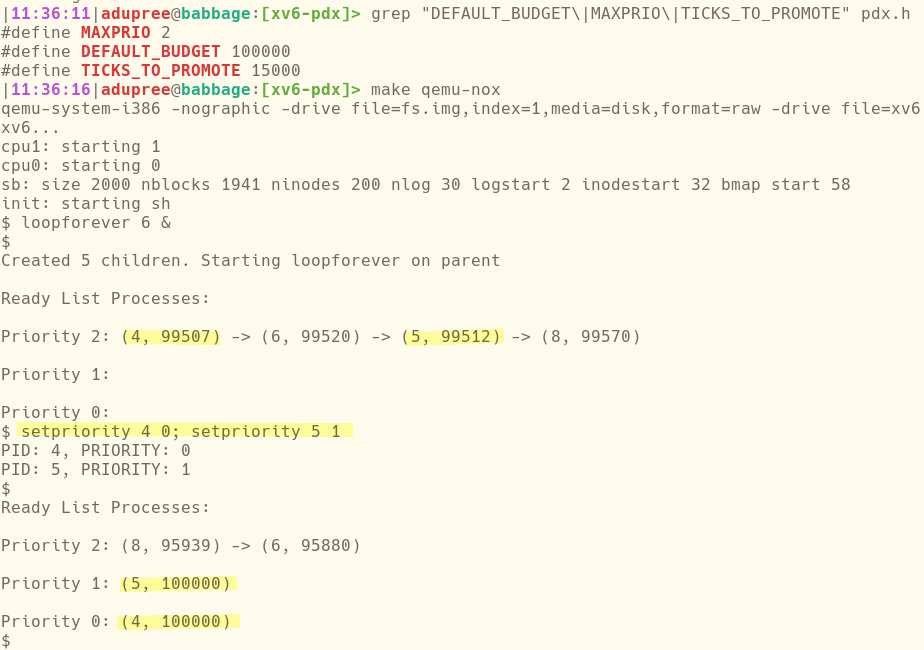
\includegraphics[width=1\linewidth]{maxprio-2-lists1.png}
	\caption[img]{Creating 6 background processes and changing priority of a couple of processes}
	\label{fig:P1compileP0-1}
  \end{figure}

  \begin{figure}[h!]
	\centering
	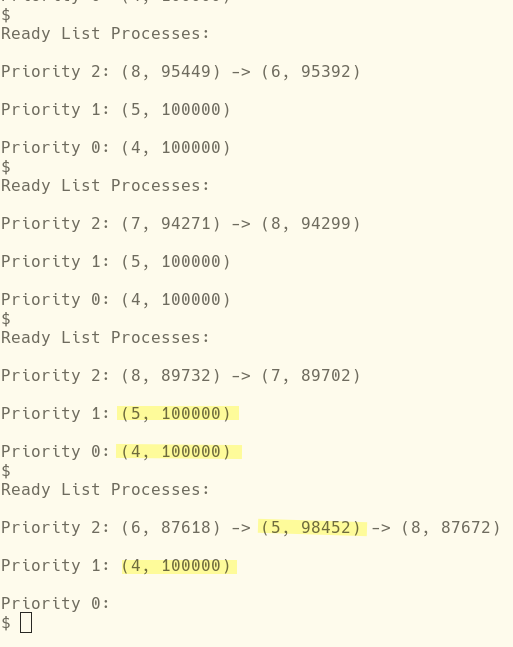
\includegraphics[width=1\linewidth]{maxprio-2-lists2.png}
	\caption[img]{Repeteadly using CTRL+R until a promotion occurs}
	\label{fig:P1compileP0-1}
  \end{figure}

  The commands in Figures 10 and 11 occur in the same session and have the \code{DEFAULT\_BUDGET}
  set to a value much greater than \code{TICKS\_TO\_PROMOTE} effectively turning off demotions in 
  the scheduler. With this setup we use \code{loopforever 6 \&} to instantiate 6 background 
  processes, that will stay in the \code{MAXPRIO} queue because the budget is so high. Then 
  we set the priority of process \code{4} to 0 and process \code{5} to 1, which correctly 
  moves them to the respective ready list. Then in Figure 11 we repteadly invoke CTRL+R until a 
  promotion occurs. First, note that the budgets for process \code{5}, and \code{4} remain unchanged.
  This is because the Scheduler always selects the first process on the highest priority non-empty 
  list. With the default budget set so high, the lower priority processes effectively 
  get starved out until they're promoted back to \code{MAXPRIO}. On the last invocation of CTRL+R we 
  can see the promotion correctly moves all processes to the next higher priority list. 

  \begin{figure}[h!]
	\centering
	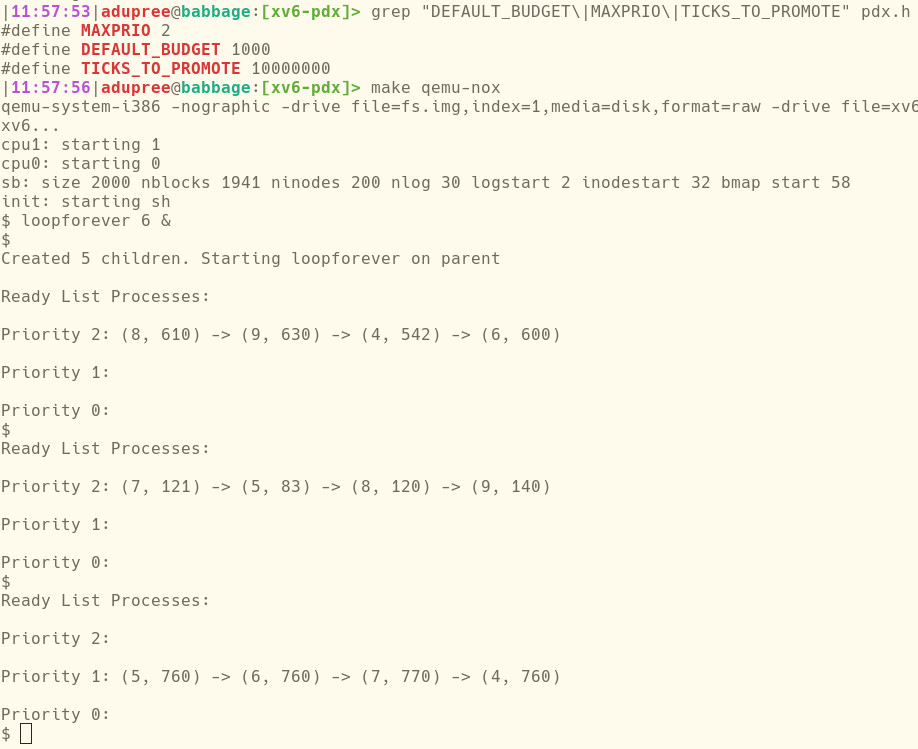
\includegraphics[width=1\linewidth]{maxprio-2-lists3.png}
	\caption[img]{CTRL+R until a demotion occurs}
	\label{fig:P1compileP0-1}
  \end{figure}

  Lastly, to prove demotion is executing properly, in Figure 12, we set the \code{DEFAULT\_BUDGET} to 1000 and 
  \code{TICKS\_TO\_PROMOTE} to a really large number, effectively turning off promotions. We can 
  see in Figure 12 that after the budgets of the background processes expire, they get moved 
  down to the next lower priority list and their budgets are reset. 

  \pagebreak

  \noindent\textbf{Test Case:} \emph{With MAXPRIO set to 6}
  
  \noindent\textbf{Assertions:}
  \begin{enumerate}[]
  \item Scheduler always selects the first process on the highest priority non-empty list
  \item Promotion correctly moves processes to the next higher priority list. 
  \item Demotion correctly moves a process to the next lower priority list.
  \end{enumerate}  
  
  \noindent\textbf{Status:} \textcolor{ForestGreen}{\textbf{PASS}}\\
  
  \begin{figure}[h!]
	\centering
	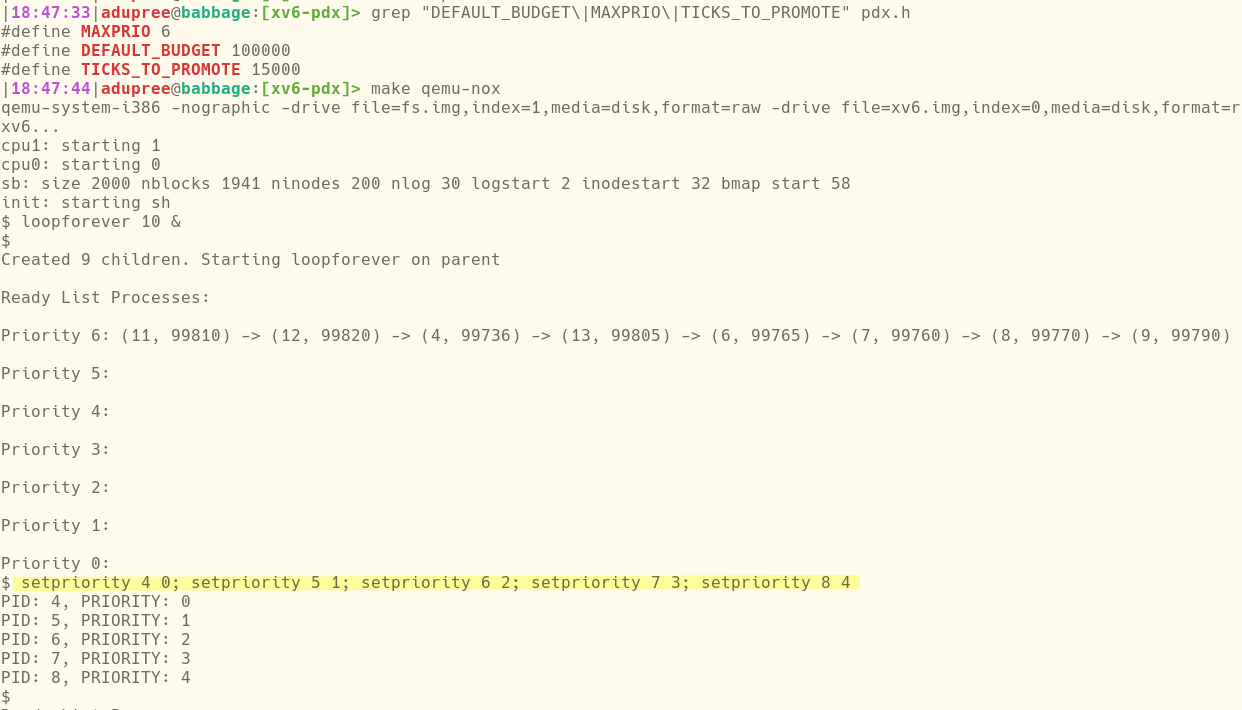
\includegraphics[width=1\linewidth]{maxprio-6-lists1.png}
	\caption[img]{Creating 10 background processes and modifying priorities}
	\label{fig:P1compileP0-1}
  \end{figure}

  \begin{figure}[h!]
	\centering
	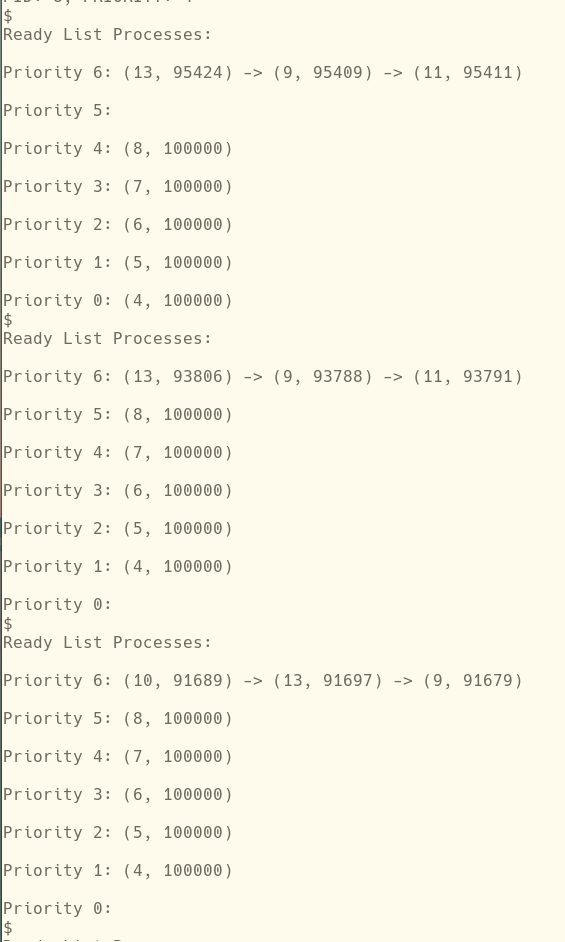
\includegraphics[scale=.75]{maxprio-6-lists2.png}
	\caption[img]{CTRL+R before and after periodic promotion}
	\label{fig:P1compileP0-1}
  \end{figure}

  \pagebreak

  Similar to the previous test case, we first use \code{grep} to verify the values of \code{MAXPRIO}, 
  \code{DEFAULT\_BUDGET}, and \code{TICKS\_TO\_PROMOTE}; which are set to 6, 100000, and 15000
  respectively. Again, because the budget is so high we are effectively turning off demotions
  in the scheduler. After instantiating 10 background processes we set the priority of processes 
  \code{4} through \code{8} to priority 0 to 4 respectively. Then, in Figure 14 we immeidiately 
  inovoke CTRL+R to show that these processes were successfully added to the correct ready list. 
  After, we wait some time for a promotion to occur and then hit CTRL+R again. As we can see in 
  Figure 14 every process (except those in \code{MAXPRIO} queue) were promoted up one level. We 
  can also deduce that the scheduler is still only selecting the first process on the highest priority
  non-empty list because the budgets for the lower priority processes remain unchanged after each
  iteration of CTRL+R. 

  \begin{figure}[h!]
	\centering
	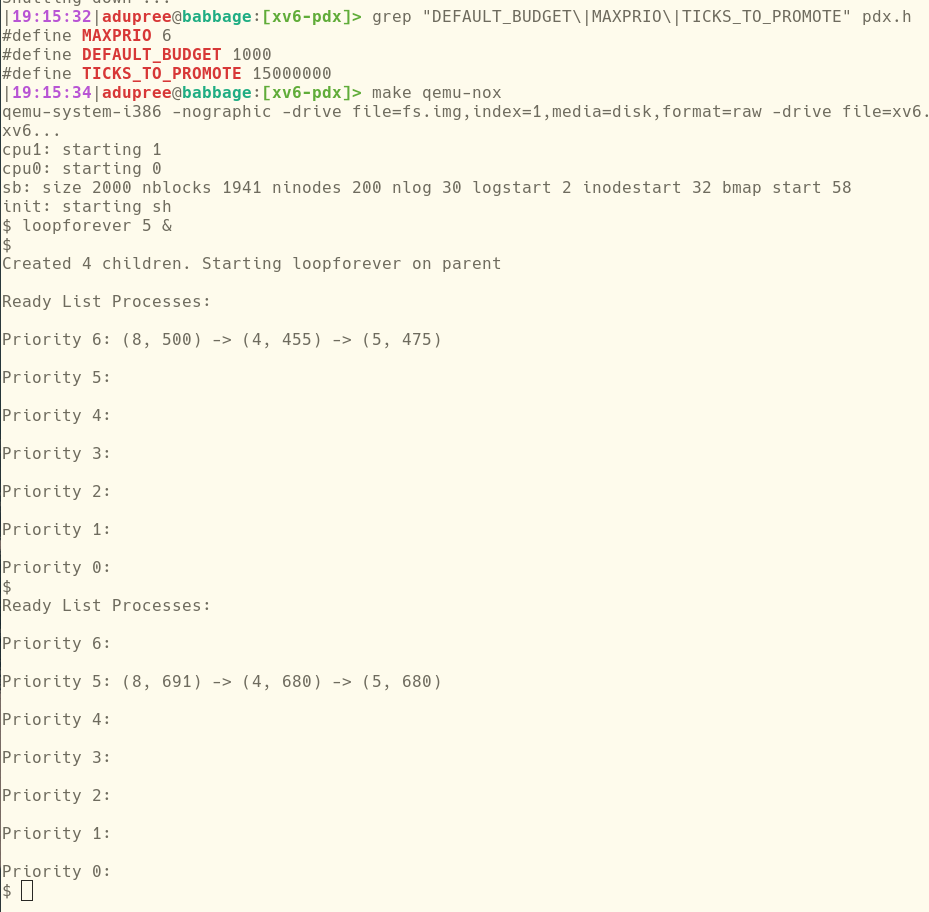
\includegraphics[width=1\linewidth]{maxprio-6-lists3.png}
	\caption[img]{Checking for correct demotion}
	\label{fig:P1compileP0-1}
  \end{figure}

  Lastly, to demonstrate demotion is occuring properly we configure the \code{DEFAULT\_BUDGET}
  to be 1000 and \code{TICKS\_TO\_PROMOTE} to be extremely large. Then after instantiating some 
  background processes we wait for the budgets to expire and a demotion to occur, at which point 
  we use CTRL+R to confirm that demotion correctly moves a process to the next lower priority list.

\ifdefined \LF
} % large print end
\fi

\end{document}